% !TEX root = ../main.tex

\section{Recognition Time}
\label{sec:results-recognition}

\scaffold{
  \textbf{Paragraph 1, setup.} Channel~1 on the tip switch and channel~2 on the ring of one jack, 10X probes, trigger on the tip switch rising through \qty{1.9}{\volt} (the plug lifting it), \qty{500}{\milli\second} window, at least 1~million points. The drive pattern of the jack changes with every state, so the ring voltage shows the phases of the jack monitor directly: the latch edges of the shift register mark where one phase ends and the next begins. The switch into following is not visible, because following keeps the drives of the last pair; it is inferred as one pair length (\qty{14.6}{\milli\second}) after the last edge. Five plug-ins and three unplugs were captured.
}

\scaffold{
  \textbf{Paragraph 2, plug-in with fresh rails.} Walk through \cref{fig:plug-in-fresh} along its labelled phases: waiting for the next plug check, the three pairs (ring pulled low at \qty{0.28}{\volt}, floating at the star point, pulled high), then following. Present \cref{tab:plug-in}: the plug was noticed 4.9 to \qty{47.3}{\milli\second} after insertion, as expected from a check every \qty{50}{\milli\second}; identification took 44 to \qty{48}{\milli\second}; in total 65 to \qty{95}{\milli\second}. A pair sometimes takes \qty{18.8}{\milli\second} instead of \qty{14.7}{\milli\second}, one extra conversion for the plug check of the other jack on the same ADC. The first run is a useful edge case: the plug was noticed before it was fully seated, tip and ring were shorted, the first pair was rejected and repeated, and the result was still correct after \qty{65}{\milli\second}.
}

\begin{figure}[htbp]
  \centering
  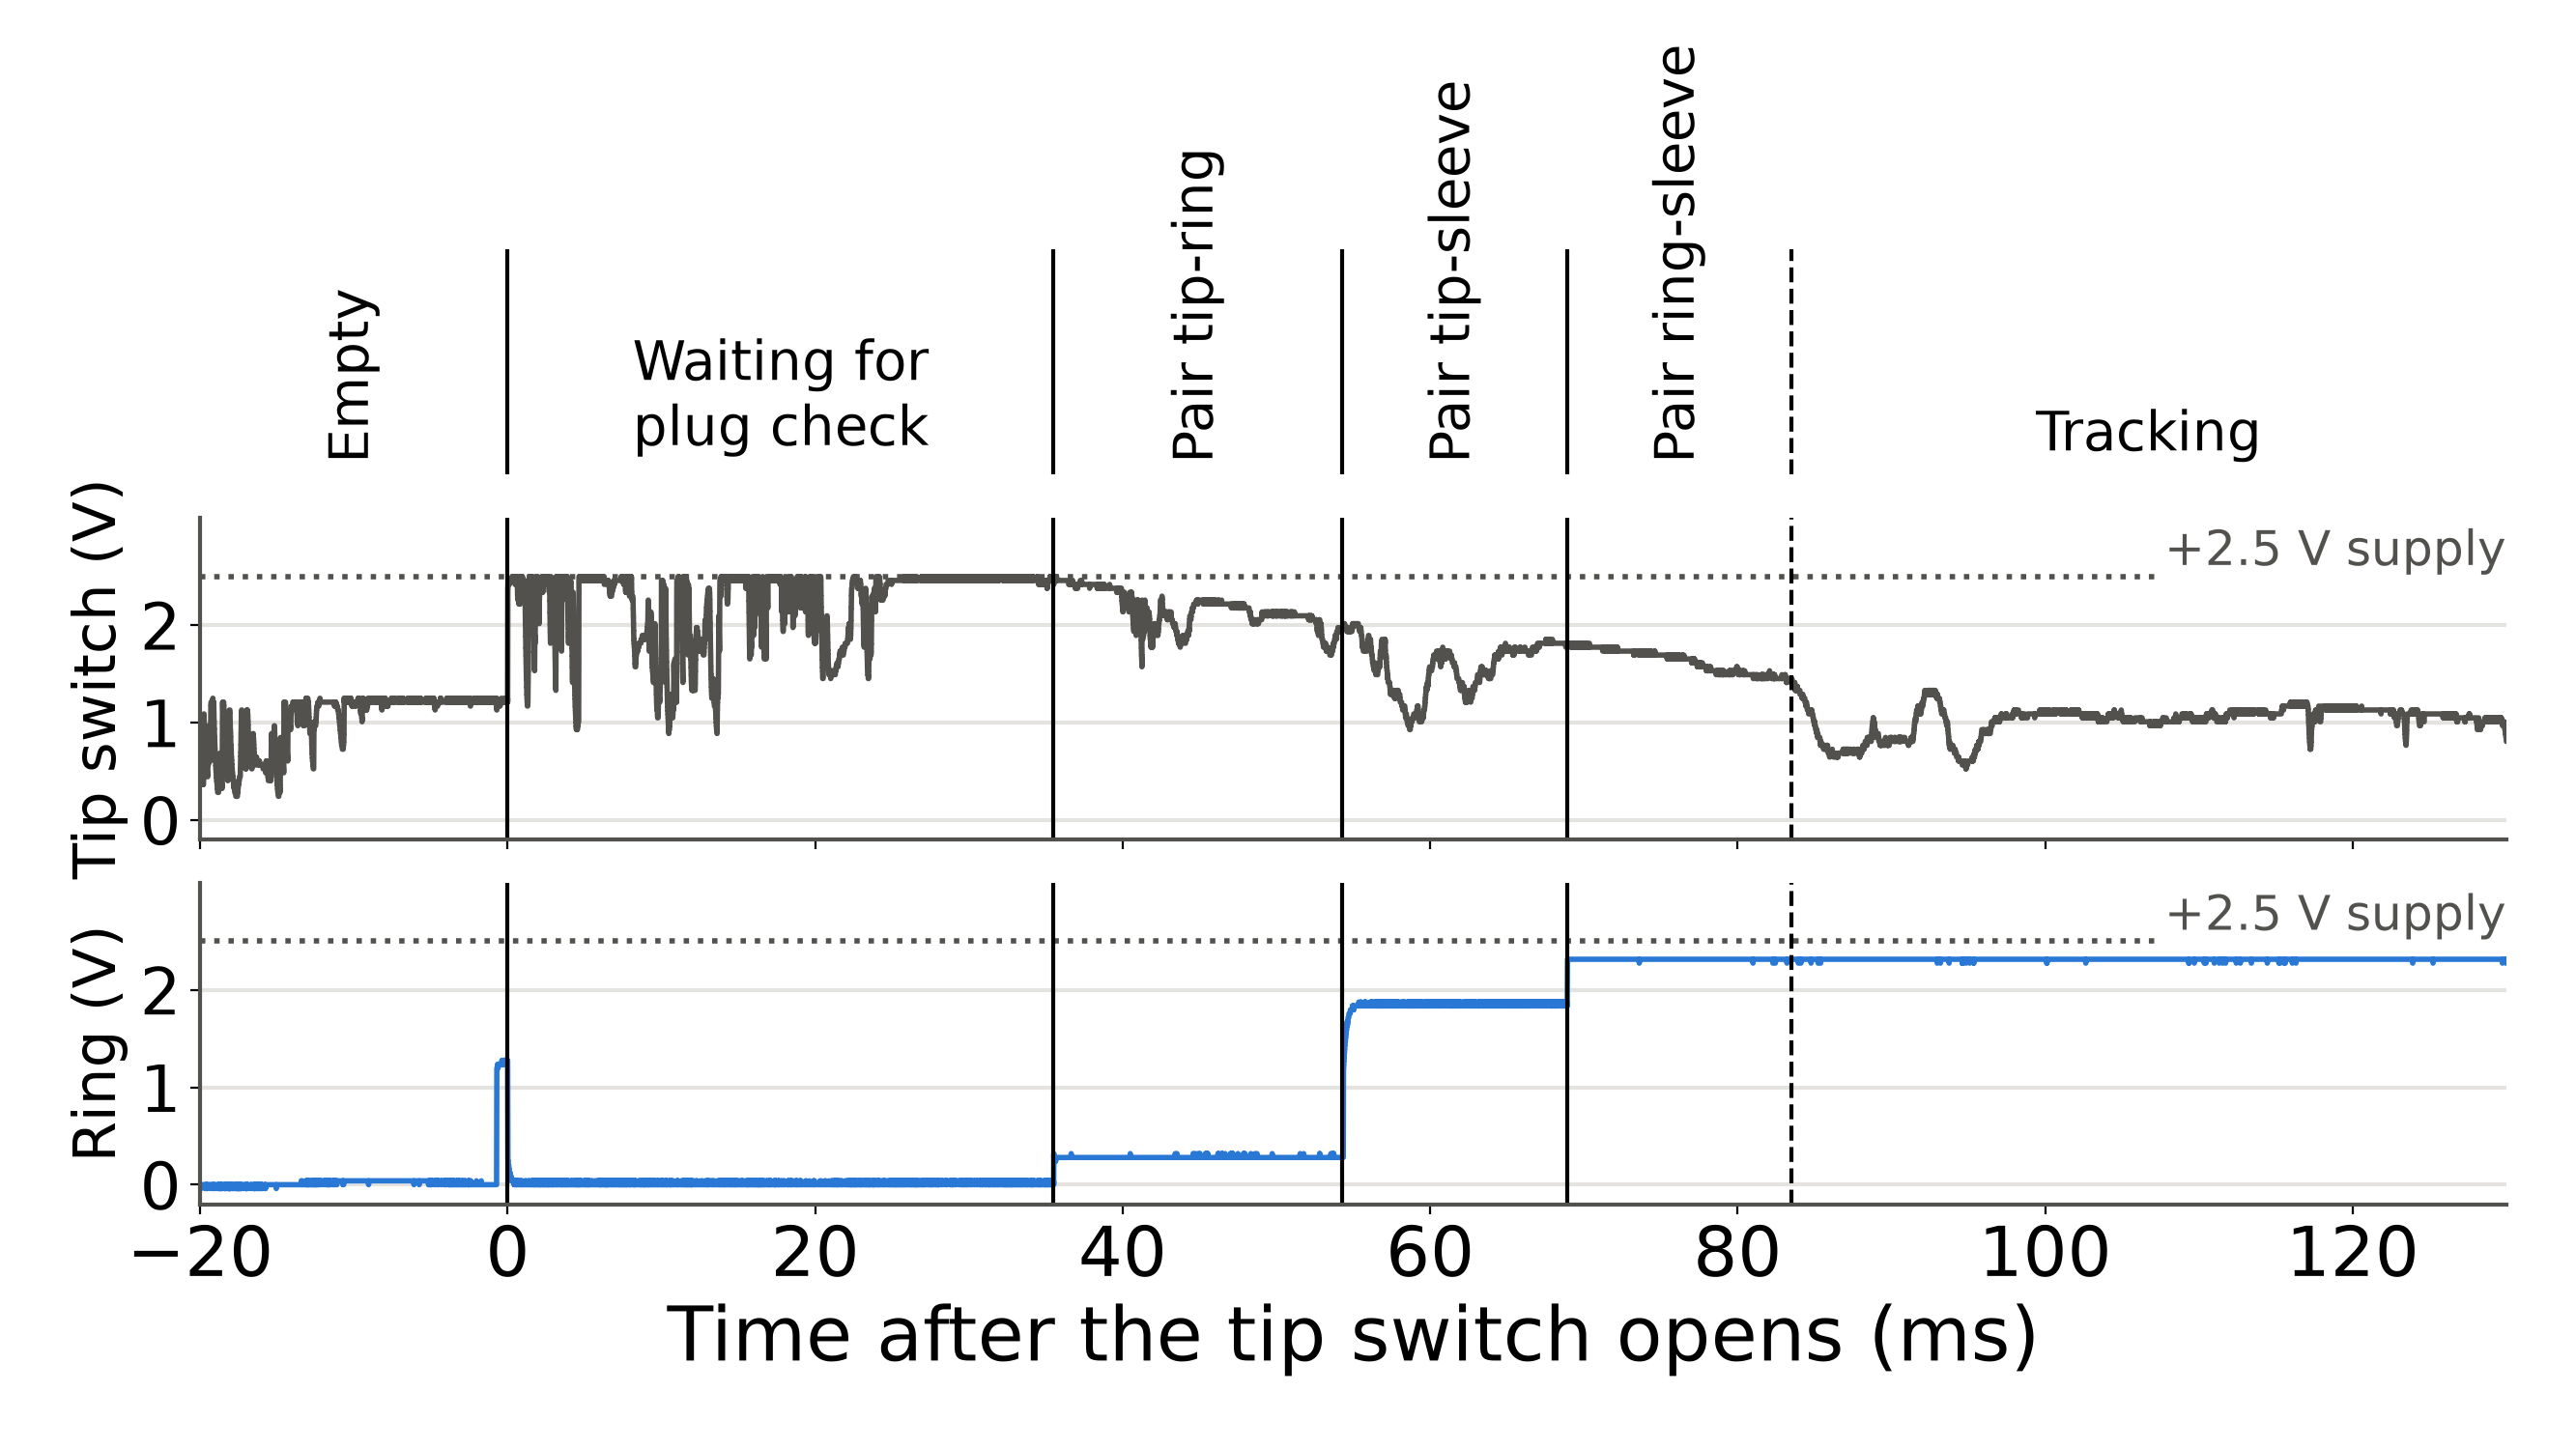
\includegraphics[width=\linewidth]{05-results/figures/plug-in-fresh-rails}
  \titledcaption{Plug-In with Fresh Rails}{\scaffoldinline{Conditions (tip switch and ring of jack~1, 10X, trigger on the tip switch at \qty{1.9}{\volt}, rails measured less than \qty{30}{\second} before); the vertical lines are latch edges, the dashed one is inferred. Capture \code{plugin5.csv}; source \code{measurements/create\_plots.py}.}}
  \label{fig:plug-in-fresh}
\end{figure}

\begin{table}[htbp]
  \centering
  \titledcaption{Plug-In Timing}{\scaffoldinline{Times in milliseconds after the tip switch opened, except the column \enquote{first pair}, which gives its duration; the start of following is inferred as the last latch plus one pair length.}}
  \label{tab:plug-in}
  \begin{tabular}{@{}lrrrr@{}}
    \toprule
    \textbf{Run} & \textbf{Plug noticed} & \textbf{First pair} & \textbf{Last latch} & \textbf{Following} \\
    \midrule
    1 & 4.9 & 31.2 (repeated) & 50.9 & $\approx$ 65 \\
    2 & 47.3 & 18.8 & 80.7 & $\approx$ 95 \\
    3 & 45.6 & 14.7 & 75.0 & $\approx$ 90 \\
    4 & 17.6 & 18.9 & 51.1 & $\approx$ 66 \\
    5 & 35.5 & 18.8 & 68.9 & $\approx$ 84 \\
    \midrule
    Rails older than \qty{30}{\second} & 49.4 & 14.7 & 292.7 & $\approx$ 300 \\
    \bottomrule
  \end{tabular}
\end{table}

\scaffold{
  \textbf{Paragraph 3, plug-in with a rail refresh.} The rails are re-measured before a solve if they are older than \qty{30}{\second}. \Cref{fig:plug-in-refresh} shows this worst case: the plug check came just before the insertion (\qty{49.4}{\milli\second} of waiting), the rails took \qty{213.8}{\milli\second} (48 readings of \qty{4.45}{\milli\second}, all arms high, then all low), and the pairs about \qty{30}{\milli\second} to \qty{44}{\milli\second}: about \qty{300}{\milli\second} in total. Mention that the pair voltages of this run differ from the other five because the wiper contact resistance changed between the pairs, and that the solver still accepted the result.
}

\begin{figure}[htbp]
  \centering
  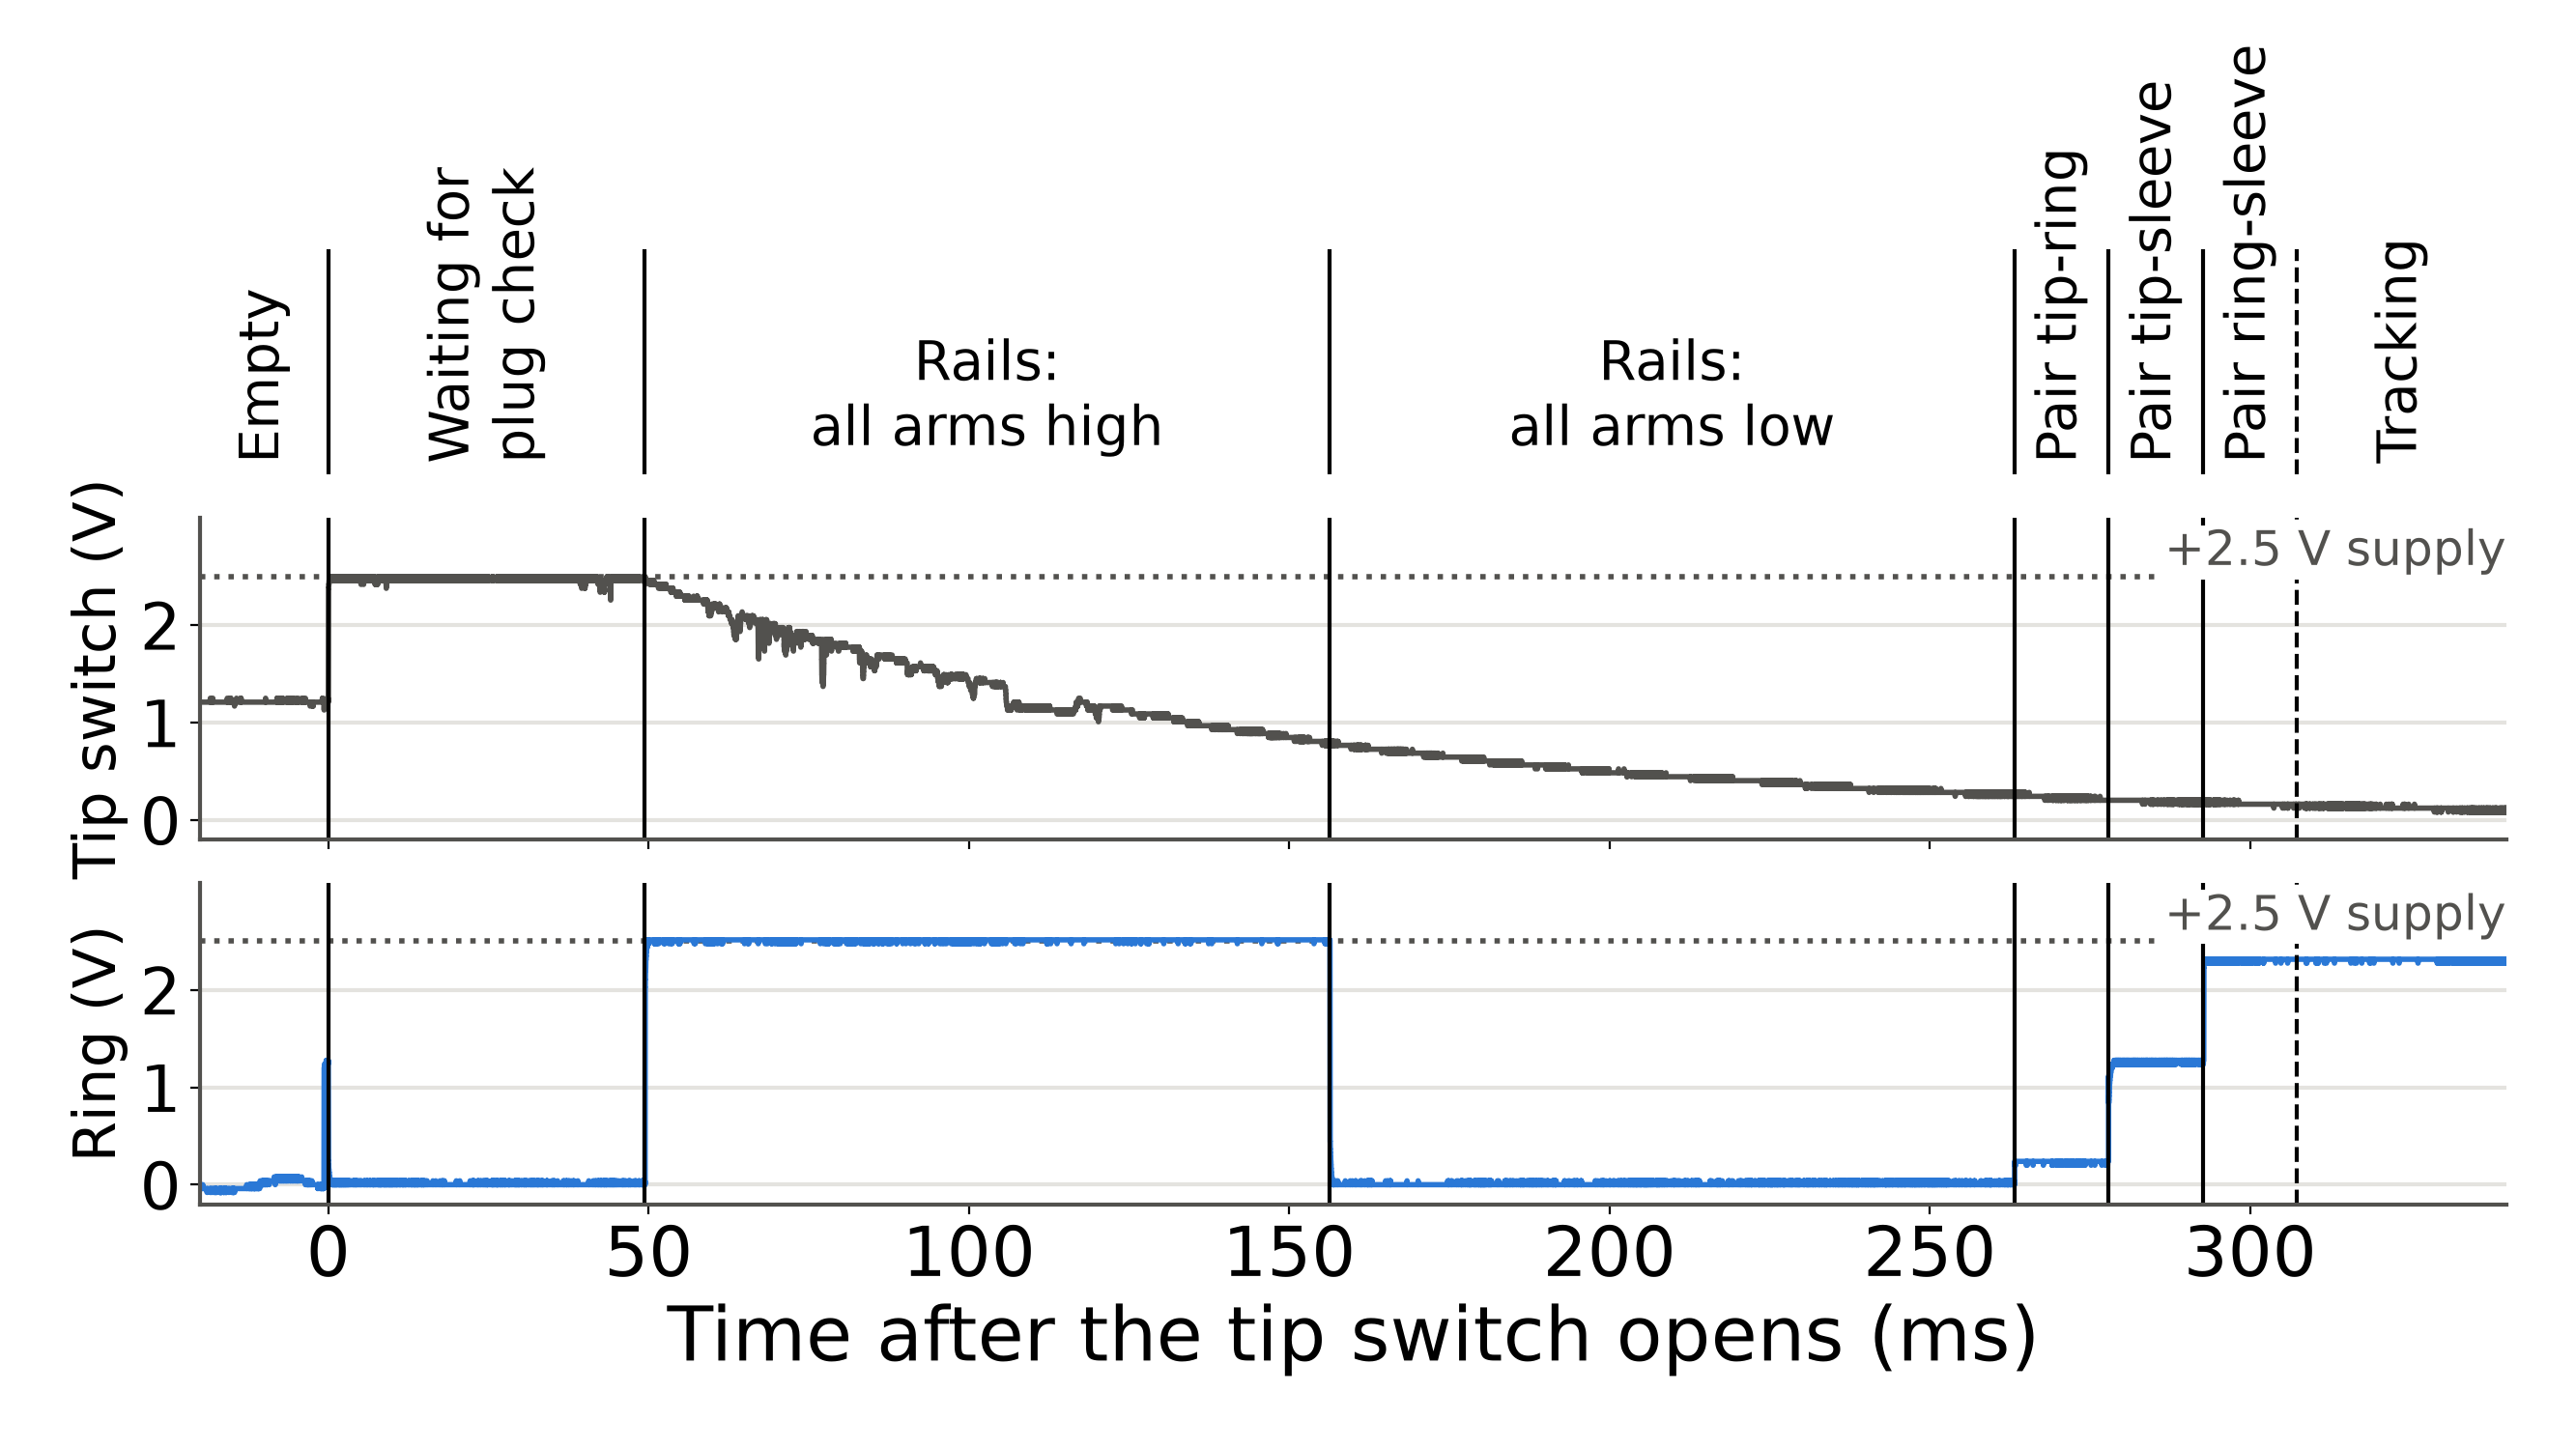
\includegraphics[width=\linewidth]{05-results/figures/plug-in-rail-refresh}
  \titledcaption{Plug-In with Rail Refresh}{\scaffoldinline{Same conditions as \cref{fig:plug-in-fresh}, but the rails were older than \qty{30}{\second}; name the two rail phases. Capture \code{plugin\_w\_rail\_meas.csv}.}}
  \label{fig:plug-in-refresh}
\end{figure}

\scaffold{
  \textbf{Paragraph 4, unplug.} \Cref{fig:unplug} (trigger on the tip switch closing): the ring loses the pedal's current about \qty{2}{\milli\second} before the tip switch closes; the firmware drops the pedal 2 to \qty{27}{\milli\second} later, re-measures the rails (about \qty{214}{\milli\second}, since the pedal had been followed for longer than \qty{30}{\second}), solves, finds no current, and the plug check reports the jack empty after 260, 330 and \qty{391}{\milli\second} in the three runs. In two of three runs a second solve was needed, because the first one saw a current just above the conduction threshold. Conclude that the rail refresh dominates both the worst-case plug-in and the unplug time.
}

\begin{figure}[htbp]
  \centering
  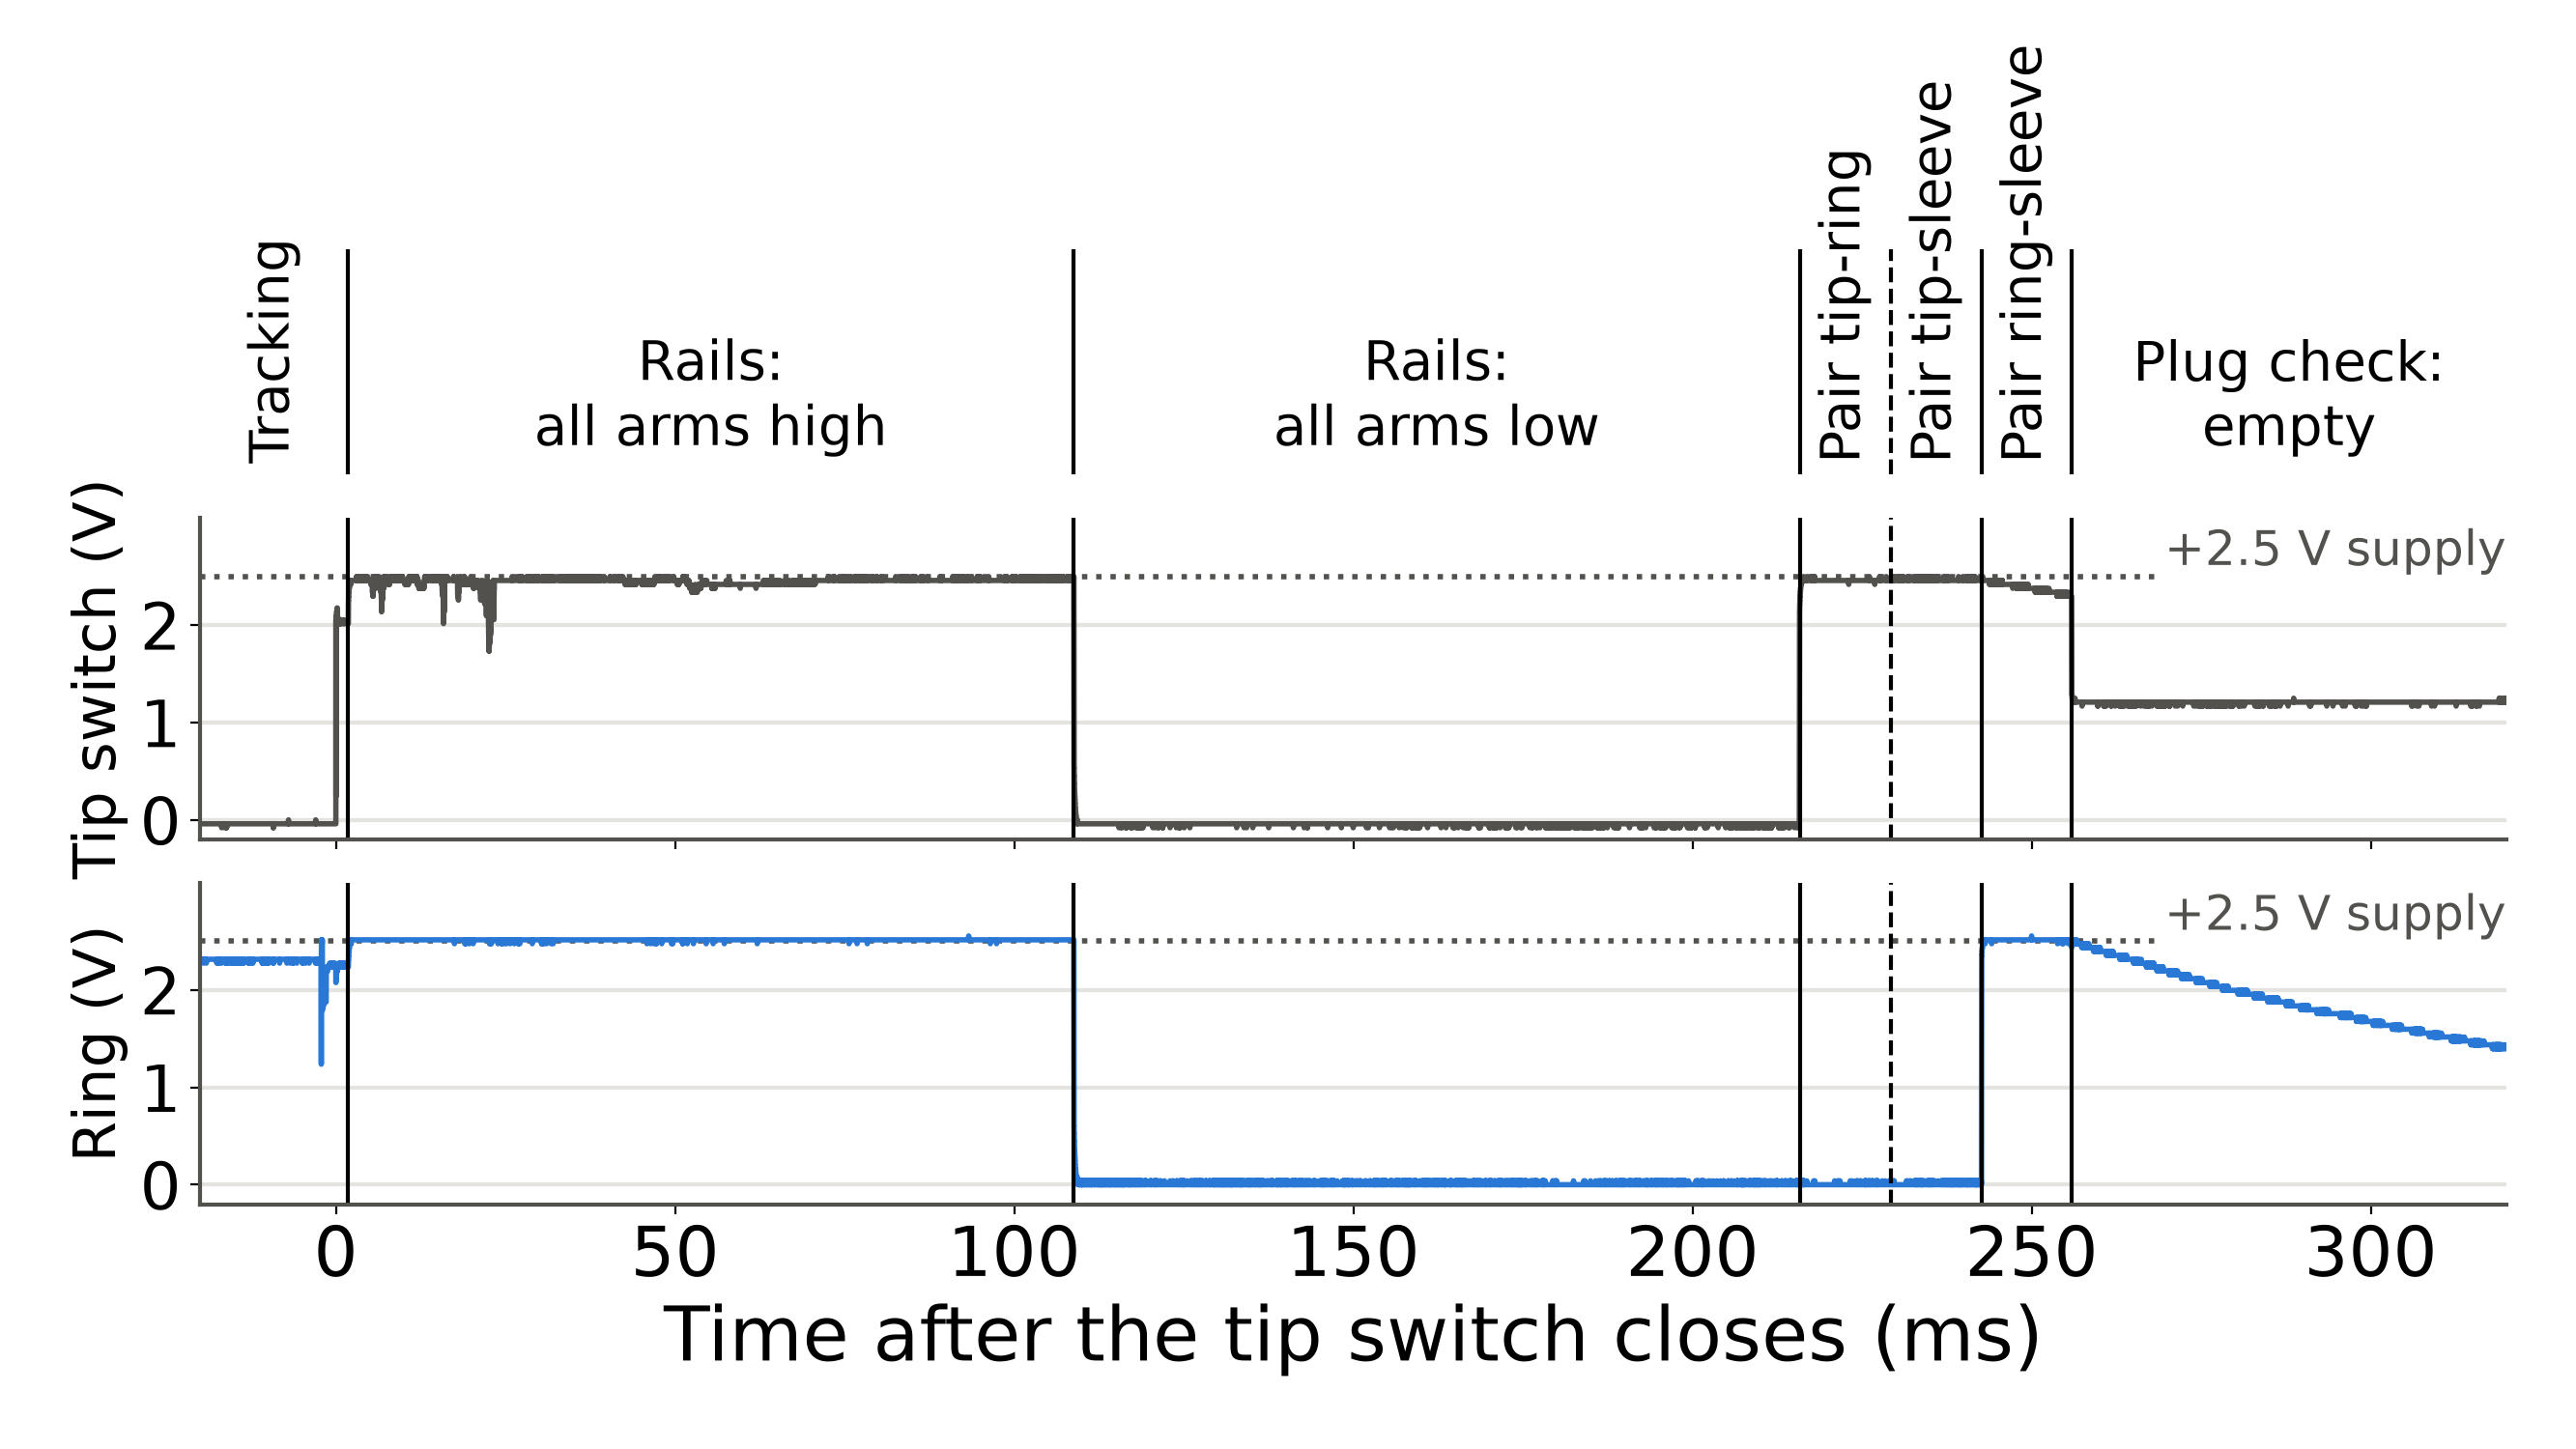
\includegraphics[width=\linewidth]{05-results/figures/unplug}
  \titledcaption{Unplug}{\scaffoldinline{Conditions (trigger on the tip switch closing); phases following, rails, three pairs, plug check; the dashed line is inferred. Capture \code{unplug1.csv}, the only run with a single solve.}}
  \label{fig:unplug}
\end{figure}
